\documentclass{article}
\usepackage{fullpage}
\usepackage{amsmath, amssymb}
\usepackage[hidelinks]{hyperref}
\usepackage[utf8]{inputenc}
\usepackage{natbib}
\usepackage{graphicx}
\usepackage{enumitem}
\usepackage{listings}
\bibliographystyle{plainnat}
% \usepackage[T1]{fontenc}


\newcommand{\R}{\mathbb{R}}
\newcommand{\Q}{\mathbb{Q}}
\newcommand{\Z}{\mathbb{Z}}
\newcommand{\N}{\mathbb{N}}
\newcommand{\C}{\mathbb{C}}

\renewcommand{\P}{\mathbb{P}}
\newcommand{\E}{\mathbb{E}}
\newcommand{\var}{\mathop{\mbox{Var}}}
\newcommand{\cov}{\mathop{\mbox{cov}}}
%\newcommand{\det}{\mathop{\mbox{det}}}
\newcommand{\supp}{\mathop{\mbox{supp}}}
\newcommand{\sgn}{\mathop{\mbox{sgn}}}
\newcommand{\EE}[1]{\E\!\left[#1\right]}
\newcommand{\PP}[1]{\P\!\left\{#1\right\}}
\newcommand{\PPP}[2]{\P_{#1}\!\left\{#2\right\}}
\newcommand{\EEE}[2]{\E_{#1}\!\left[#2\right]}
\newcommand{\EEsup}[2]{\E^{#1}\!\left[#2\right]}

\newcommand{\bone}{\mathbf{1}}

% These macros are borrowed from TAOCPMAC.tex
\newcommand{\slug}{\hbox{\kern1.5pt\vrule width2.5pt height6pt depth1.5pt\kern1.5pt}}
\def\xskip{\hskip 7pt plus 3pt minus 4pt}
\newdimen\algindent
\newif\ifitempar \itempartrue % normally true unless briefly set false
\def\algindentset#1{\setbox0\hbox{{\bf #1.\kern.25em}}\algindent=\wd0\relax}
\def\algbegin #1 #2{\algindentset{#21}\alg #1 #2} % when steps all have 1 digit
\def\aalgbegin #1 #2{\algindentset{#211}\alg #1 #2} % when 10 or more steps
\def\alg#1(#2). {\medbreak % Usage: \algbegin Algorithm A (algname). This...
  \noindent{\bf#1}({\it#2\/}).\xskip\ignorespaces}
\def\kalgstep#1.{\ifitempar\smallskip\noindent\else\itempartrue
   \hskip-\parindent\fi
   \hbox to\algindent{\bf\hfil #1.\kern.25em}%
   \hangindent=\algindent\hangafter=1\ignorespaces}

\newcommand{\algstep}[3]{\kalgstep #1 [#2] #3 }
\newenvironment{taocpalg}[3]{%
\vspace{1em}%
\algbegin Algorithm #1. ({#2}). #3 }
{\vspace{1em}}

\newcommand{\randomuniform}[0]{\mathcal{R}_U}
\newcommand{\randomdiscrete}[0]{\mathcal{R}_D}
\newcommand{\algref}[1]{#1}

% \newcommand{\tablenotation}[1]{\mathcal{#1}}
% \newcommand{\tableaddrow}[0]{\mbox{add}}


\newcommand{\msprime}{\texttt{msprime}}
\newcommand{\nodes}{\texttt{nodes}}
\newcommand{\edgesets}{\texttt{edgesets}}
\newcommand{\sites}{\texttt{sites}}
\newcommand{\mutations}{\texttt{mutations}}

\usepackage{color}
\newcommand{\plr}[1]{{\em \color{blue} #1}}

\begin{document}

\title{Efficient forwards-time simulation with ancestral recombination graphs}
\author{Jerome Kelleher, 
        Kevin R. Thornton,
        Jaime Ashander, and
        Peter L. Ralph}
\maketitle

\emph{Note:} author order not determined

\begin{abstract}
    To use genomic data for inference and prediction 
    it is often necessary to obtain whole-genome information
    from individual-based simulations,
    but the computational burden of tracking the genome of each simulated individual can be substantial.
    In this note we describe how to both (a) dramatically reduce this burden and 
    (b) efficiently record the entire history of the population.
    We do this by simulating only those loci that may affect reproduction (those having non-neutral variants),
    and recording the entire history of genetic inheritance in an efficient representation of the ancestral recombination graph,
    on which neutral mutations can be quickly placed afterwards.
    \plr{make more clear data structure was already developed? refer to 'tree sequence' by name?}
    The algorithm is implemented in python,
    and is designed to be easily used by any forwards-time simulation software.

    Coalescent simulations are very helpful but require random mating and neutrality.
    For continuous space, polygenic selection, or detailed dissection of life history, 
    we must use forwards-time, individual-based simulation.
    These are much slower due in part to carrying around neutral genotypes irrelevant to the process.
    Here we show how to efficiently produce and store the entire history of ancestry and recombination
    (the ARG) from an individual-based simulation,
    on which neutral mutations can be placed afterwards.
    This has the promise of making large-scale, whole-genome simulations with realistic geography and selection finally possible.
\end{abstract}


\textbf{OUTLINE}
\begin{enumerate}
    \item motivate need for whole-genome fwd-time simulations; point out that we only recently have the computing power to do this
    \item explain ARG: explain that for forwards-time only need selected loci as by defn all others can be put on afterwards
    \item review something about msprime methods for storing/traversing tree sequence
    \item describe tables and write out conditions to have valid tables
    \item write down algorithm used to do simple WF simulation
    \item describe simplify algorithm
    \item back-of-the-envelope calculation to compare cost of tracking whole genomes versus putting mutations on ARG
    \item comparison of speed with simupop, fwdpp
\end{enumerate}


%%%%%%%%%%%%%%%%%%%%%%
\section*{Introduction}

\plr{perhaps some of this veers into methods rather than introduction}

Since the 1980's, coalescent theory has enabled computer simulation of the results of population genetics models
identical to that which would be produced by large, randomly mating populations over long periods of time
without actually requiring simulation of so many generations or meioses.
Coalescent theory thus had three transformative effects on population genetics:
first, giving researchers better conceptual tools to describe \emph{gene trees} and thus bringing within-population trees into better focus;
second, producing analytical methods to estimate parameters of interest from genetic data (e.g. $\theta = 4N_e \mu$);
and finally, providing a computationally feasible method to produce computer simulations of population genetics processes.
However, these powerful advances came with substantial caveats:
the backwards-in-time processes that are described by coalescent theory
are only \emph{Markovian}, and thus feasible to work with,
thanks to the important assumptions of (a) random mating, and (b) neutrality.
\plr{Brief statement why this is.  Also include stationarity?}
Both assumptions can be side-stepped to a limited extent, and so coalescent methods are now commonly used to
simulate the results of population dynamics of a collection of randomly mating populations exchanging migrants,
having a small number of loci under selection.
Mapping results of such models onto real species can be challenging,
as these are often distributed across geographical space and may have large numbers of loci under various sorts of selection.
Furthermore, the relationship between the life history of a species --
fecundity and mortality schedules, allee effects, and demographic fluctuations --
are all absorbed into a single compound parameter, the coalescence rate.
These considerations, and increasing computational power, have led to a resurgence of interest in forwards-time, individual-based simulations.

With modern computing power, pure demographic calculations are not a barrier,
even though biological population sizes are often above $10^6$,
and coalescent theory tells us that a population of size $N$ 
must be run for a multiple of $N$ generations to produce stable genetic patterns.
However, if our interest lies in the resulting genetic patterns of variation
-- and often, the point of such simulations is to compare to real data --
then such simulations must somehow produce at the end data for each individual on a genomic scale.
As samples of most species genomes harbor tens or hundreds of millions of variant sites,
naively carrying full genotypes for even modest numbers of individuals through a simluation becomes quickly prohibitive.

However, it is thought that much of that variation is selectively neutral (or nearly so).
By definition, the alleles carried by individuals in a population at neutral sites
do not affect the population process.
For this reason, if one records the entire genealogical history of a population over the course of a simulation,
one can lay down neutral mutations on top of that history afterwards,
without loss of generality.
Precisely, we would need to know the genealogical tree relating all sampled individuals
at each position along the genome.
In this paper, we show how to use algorithmic tools and data structures developed for the coalescent simulator \msprime
to efficiently record, and later process, this history.

In so doing we record the \emph{population pedigree} --
the entire history of parent-offspring relationships of an entire population going back to a remote time --
as well as information encoding the genetic outcomes of each ancestral meiosis --
who inherited which parts of which parental chromosomes.
This embellished graph is known as the \emph{ancestral recombination graph}, or {ARG} \citep{griffiths}.
Combined with ancestral genotypes and the origins of new mutations,
it completely specifies the genomic sequence of any individual in the population at any time.
However, much less than the entire ARG is needed to specify relationships 
between any given set of samples --
only those portions of it from which those samples have actually inherited, 
back to their most recent common ancestors.
The assumptions of coalescent theory 
% -- random mating and neutrality --
imply that this random set describes a Markov process looked at \emph{backwards} in time,
and can hence be simulated without reference to the unnecessary remainder 
\citet{griffithsmarjoram,msprime}.
This stochastic process is also called the ``ARG'',
but we reserve this name for the embellished graph itself.
% Although this point was in principle known since \citet{griffithsmarjoram},
% only recent algorithmic advances made it possible to actually simulate the process correctly,
% without approximation, across whole chromosomes \citep{msprime}.



%%%%%%%%%%%%%%%%%%%%%%
\section*{Methods}

\plr{Reminder of what we need to know in the end (the trees), and
    quick review of \msprime{} methods: sparse trees, tree differences.}

%%%%%%
\subsection*{Data structures:}

First we describe the data structures we use for recording genealogical history,
as implemented in \msprime{}.
These derive from those described in \citet{msprime},
but have been modified to remove redundancy.
The tables below give the example tree sequence of Figure \ref{fig:ex_tree_seq}.

\begin{figure}
    \begin{center}
        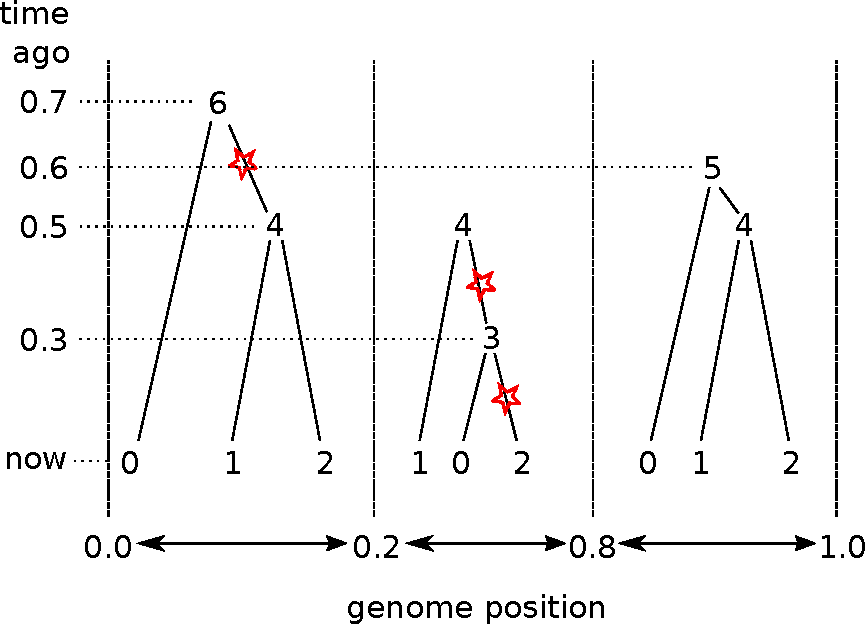
\includegraphics[width=0.6\textwidth]{example_tree_seq}
    \end{center}
    \caption{
        A pictorial representation of the ARG
        relating three samples to each other
        over a chromosome of length 1.0.
        Mutations shown in the example tables of the text
        are marked with red stars.
        \label{fig:ex_tree_seq}
    }
\end{figure}

To clarify terminology,
below a \emph{tree} refers to
a genealogical tree describing how a collection of individuals are related to each other.  
A \emph{tree sequence} contains information sufficient to reconstruct the genealogical
tree relating all samples to each other at any point along the genome.
In the context of a tree sequence,
\emph{nodes} refer to distinct ancestors,
and may be identified with points in the trees of a tree sequence.
Every tip or branching point in a tree is associated with a node.
A tree sequence does not necessarily carry complete genealogical information about every node,
but calling a node a \emph{sample} implies that complete information is present for that ancestor,
i.e., the node is associated with a point in every tree in the tree sequence.
Since each node represents a certain ancestor, it has a
unique ``time'', thought of as her birth time, which determines the height
of any branching points she is associated with.  A given node will be
associated with branching points of all trees across a region if that node
is the most recent common ancestor to the subtending tips across that region.  
This information is stored in the columns of a \textbf{Node Table}:
\begin{center}
\begin{tabular}{cccc}
    id   &  is\_sample &  population &  time \\
    0    &  1          & 0           & 0 \\
    1    &  1          & 0           & 0 \\
    2    &  1          & 0           & 0 \\
    3    &  0          & 0           & 0.3 \\
    4    &  0          & 0           & 0.5 \\
    5    &  0          & 0           & 0.6 \\
    6    &  0          & 0           & 0.7 \\
\end{tabular}
\end{center}
where ``flags'' records other information 
(e.g., a binary mask of `1' indicates the node is a sample).
Importantly, the \textbf{node ID} of a node is given implicitly
by the (zero-based) index of its corresponding row in the Node Table.

Tree sequences are constructed by specifying over which segments of genome
which nodes inherit from which other nodes.  This information is stored by
recording the endpoints of each distinctly inherited ancestral segment,
the parental node, and a list of children nodes who have inherited that segment.
As each such record describes a collection of edges across a swatch of trees in the tree sequence,
we call these \emph{edgesets} 
and store them in the columns of an \textbf{Edgeset Table:}
\begin{center}
\begin{tabular}{cccc}
    left & right & parent & children \\
    0.2  &  0.8  &  3     & 0,2 \\
    0.0  &  0.2  &  4     & 1,2 \\
    0.2  &  0.8  &  4     & 1,3 \\
    0.8  &  1.0  &  4     & 1,2 \\
    0.8  &  1.0  &  5     & 0,4 \\
    0.0  &  0.2  &  6     & 0,4  \\
\end{tabular}
\end{center}

To record information about genetic variants we need to also record each mutation
and which nodes have inherited that mutation.
The tree structure takes care of inheritance -- all we need to do
is to record the highest node in the tree at the mutated site
that inherited that mutation.
As more than one mtuation may occur at a given site,
we separate this information into two tables,
first, the \textbf{Site Table} records for each variant site
\begin{center}
\begin{tabular}{ccc}
    id  &   position  & ancestral\_state \\
    0   &  0.1        & 0 \\
    1   &  0.5        & 0 \\
\end{tabular}
\end{center}
Here ``position'' is a (floating point) position along the chromosome,
and ``ancestral state'' is the genotype of the root of the tree at that site.
As for nodes, \textbf{site IDs} are given implicitly
by the (zero-based) index of the rows.
Then, we record in a \textbf{Mutation Table}
\begin{center}
\begin{tabular}{ccc}
    site  & node  & derived\_state \\
    0	  & 4	  & 1 \\
    1	  & 3	  & 1 \\
    1	  & 2	  & 0 \\
\end{tabular}
\end{center}
in which ``site'' is the ID of the site at wihch this mutation occurred,
``node'' is the ID of the highest node that has inherited this mutation,
and ``derived state'' is the genotype at this site of any individuals inheriting this mutation,
unless another mutation occurs.
% \plr{Omit migrations?}

\paragraph{Definition of valid tables}
Here are the formal requirements for a set of nodes and edgesets to make sense,
and to allow ``msprime``'s algorithms to work properly.

To disallow time travel and multiple inheritance:
\begin{enumerate}
    \item Offspring must be born after their parents (and hence, no loops).
    \item The set of intervals on which each individual is a child must be disjoint.
\end{enumerate}
For algorithmic reasons, we also require:
\begin{enumerate} \setcounter{enumi}{2}
    \item The leftmost endpoint of each chromosome is 0.0.
    \item Node times must be strictly greater than zero.
    \item The list of offspring in an edgeset must be sorted.
    \item Edgesets must be sorted in nondecreasing time order.
    \item The set of intervals on which each individual is a parent must be disjoint.
    \item Each edgeset must contain at least two children.
\end{enumerate}
Note that since each node time is equal to the amount of time since the \emph{birth} of the
corresponding parent, time is measured in clock time, not in meioses.

A forwards-time simulation does \textbf{not} naturally emit genealogical information
satisfying requirements 5--8.
However, \msprime{} implements two algorithms that will take a set of tables
satisfying only 1--4 and produce tables satisfying all requirements.
Trivially, \texttt{sort\_tables} enforces requirements 5 and 6 and does not renumber nodes;
then, \texttt{simplify} enforces requirements 7 and 8 (and does much more; see below).


%%%%%%
\subsection*{Recording the ARG in forwards time}

To record the genealogical history of a simulation
we need to record two things for each new chromosome:
the birth time,
and the endpoints and parental IDs of each distinctly inherited segment.
This is recorded easily, without further processing,
in the tables described above.

For concreteness, here we write out in pseudocode
how to run a neutral Wright--Fisher simulation
with overlapping generations
that records genealogical history in this way.
The simulation will run for $T$ generations,
and has $N$ haploid individuals, each carrying a single chromosome of length L,
on which for simplicity we assume there is exactly one crossover per generation.
The probability of death per individual each generation is \texttt{death\_prob},
and the whole-chromosome mutation rate per individual is \texttt{mut\_rate}.

\paragraph{Initialize:}
We will build the tables \nodes, \edgesets, \sites, and \mutations,
and keep track of the IDs of the current generation in the list \texttt{pop}.
\begin{lstlisting}[language=Python]
for i in 0:N-1:
    nodes.add_row(time=T)
    pop[i] = i
\end{lstlisting}
(Alternatively, the tables could be initialized by the results of a coalescent simulation.)

\paragraph{Iterate:}
We then step through the generations,
using the functions \texttt{random\_mutation} and \texttt{random\_allele}
to choose positions and alleles for mutations, respectively:
\begin{lstlisting}[language=Python]
for t in 1:T:
    for i in 0:N-1:
        if random.uniform() > death_prob:
            new_pop[i] = pop[i]
        else:
            u = nodes.num_rows  # the ID of the new individual
            new_pop[i] = u
            nodes.add_row(time = T-t)
            a = random.sample(pop)
            b = random.sample(pop)
            bp = random.sample(0:L)
            if bp > 0:
                edgesets.add_row(left=0, right=bp,
                                  parent=a, children=(u,))
            if bp < L:
                edgesets.add_row(left=bp, right=L,
                                  parent=b, children=(u,))
            num_muts = random.poisson(mut_rate)
            for j in 1:num_muts:
                pos = random_mutation()
                if pos not in sites.position:
                    s = sites.num_rows
                    sites.add_row(position=pos, 
                           ancestral_state=random_allele())
                else:
                    s = sites.position.index(pos)
                mutations.add_row(site=s, node=u, 
                           derived_state=random_allele())
    pop = new_pop
\end{lstlisting}

\paragraph{Finalize:}
to obtain a tree sequence, we need only transform the tables to the required format:
\begin{lstlisting}
sort_tables(nodes, edgesets, sites, mutations)
simplify_tables(nodes, edgesets, sites, mutations)
\end{lstlisting}
which can then be loaded into a tree sequence with \msprime.
(These two functions operate on the tables in place.)



\begin{figure}
    \begin{center}
        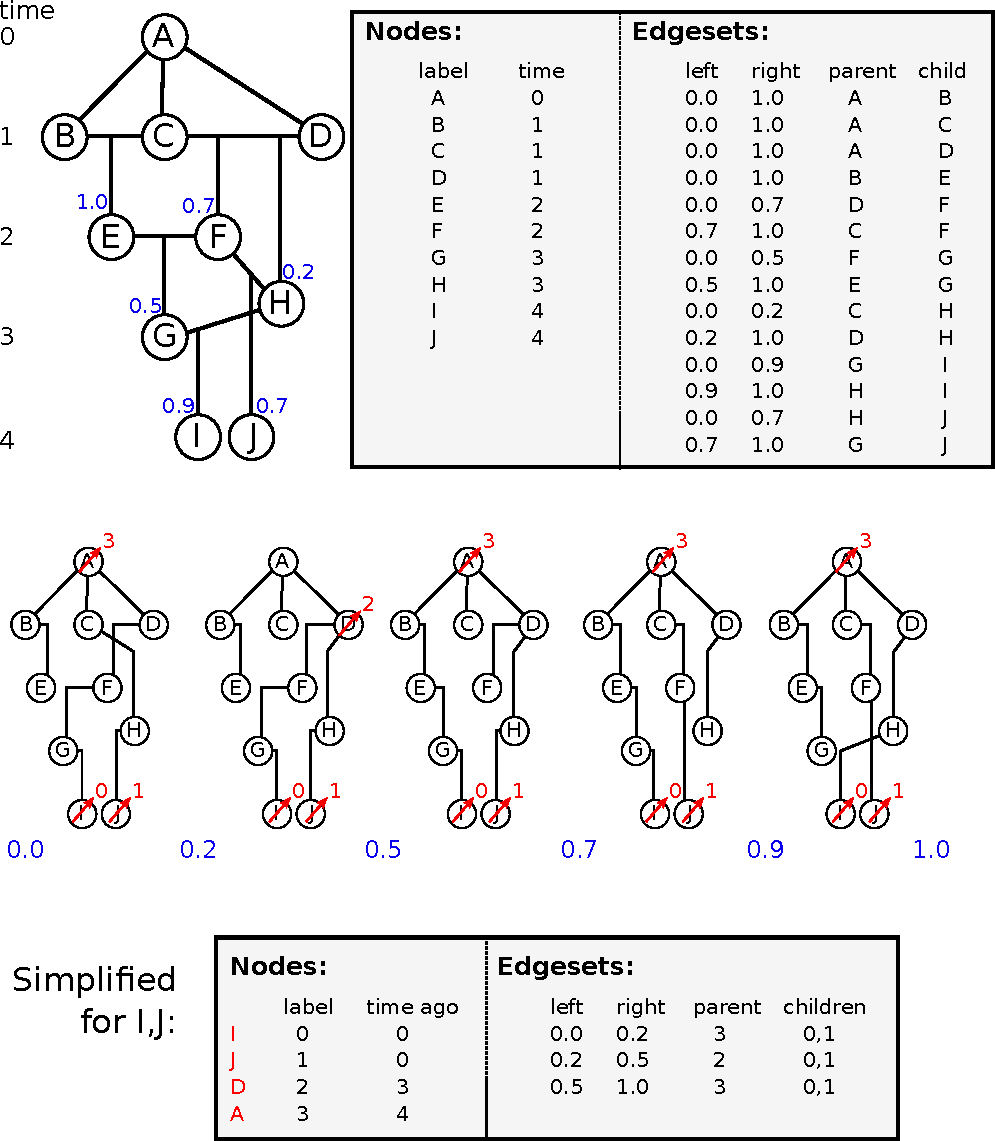
\includegraphics{method_diagram}
    \end{center}
    \caption{
        A simple example of the method.
        \textbf{Top:} the ARG shown on the left relates ten haploid individuals to each other.
        It is recorded, in forwards time, 
        in 10 node records (one for each individual)
        and 14 edgeset records (one for each distinctly inherited segment).
        Blue numbers denote crossing over locations in each meiosis.
        The individuals $B$, $C$, and $D$ inherit clonally from $A$
        to ensure rootnedness of resulting tree.
        \textbf{Center:} the five distinct trees relating all individuals to each other
        found across the chromosome (blue numbers denote locations on the chromosome).
        Labels after simplification are shown in red.
        \textbf{Bottom:} tables recording the tree sequence after simplification 
        with nodes $I$ and $J$ as samples.
        The mapping from labels in the forwards time simulation to nodes in the tree sequence
        is shown in red,
        which allows additional records to be added as the simulation progresses.
        \label{fig:method_diagram}
    }
\end{figure}


%%%%%%
\subsection*{Tree sequence simplification}

The resulting tables encode everything we need to know --
in fact, they record all of history for everyone alive at any time through the simulation.
This is much more than we need to reconstruct the genealogies and sequences
of a smaller sample of indidivuals.
Reducing this larger tree sequence to a smaller one relevant to a given set of ``sample'' nodes
we call \emph{simplification}.
Roughly, this works by tracing ancestry from the samples backwards through the recorded history,
adding node and edgeset records to the output only when coalescent events are reached.
This works exactly as in \msprime, allowing substantial re-use of algorithms;
the main difference being that parental choice, mutations, and recombination locations 
are determined by the input tree sequence
rather than randomly generated.
An example is shown in Figure \ref{fig:method_diagram}.

In this scheme,
at any point in the simulation genealogical history is recorded in a tree sequence.
This has two additional advantages.
First, simplification can be run periodically through the simulation,
taking the set of samples to be the entire currently alive population.
This is important as it keeps memory usage from growing linearly (and quickly) with time.
Second, the simulation can be \emph{begun} with a tree sequence produced by some other method --
for instance, by a coalescent simulation with \msprime.
This allows for incorporation of deep-time history beyond the reach of individual-based simulations.
Since geographic structure from times longer ago than the mixing time of migration across the range
has limited effect on modern genealogies \citep{wilkins_separation}
(other than possibly changing effective population size \citet{durretspatial}),
this may not negatively affect realism.

\plr{Something about putting mutations down on the tree sequence.}

%%%%%%
\subsection*{Overview of the API}

\plr{Quick overview of how to efficiently hook this up with other code.}


%%%%%%%%%%%%%%%%%%%%%%
\section*{Results}

\plr{Estimates of run-time complexity}
Suppose that we wish to run a forwards-time simulation of $N$ individuals for $T$ generations,
in which there are $S$ selected loci and $L$ neutral loci.
We will estimate run-time complexity and memory usage for both a ``naive'' strategy that carries along neutral loci
and an ``ancestry-tracking'' strategy like that we consider here.
To do this, we assume that each individual must carry along its entire genotype.
More advanced schemes are used in some simulators,
but these increase efficiency by utilizing redundancy introduced by shared ancestry, 
which is effectively an intermediate scheme.
We omit the cost of computing a fitness function.

Both schemes must choose mates and recombination breakpoints,
and pass on selected genotypes.
The difference between the two comes from the tradeoff between
(a) passing on neutral genotypes, and
(b) recording and simplifying the tree sequence, and adding neutral genotypes afterwards.
(We assume here that selected genotypes are stored in the same way for both.)
Passing on neutral genotypes naively records $L$ items per individual each generation, discarding the previous generation.
\plr{do this better with numbers from nodes, edgesets}
Recording a tree sequence stores 2 parents and $\rho$ breakpoints on average each generation;
after $T$ generations this grows to $N \times T \times (2 + \rho)$ stored items.
However, after simplification a tree sequence for all $N$ individuals
only takes of order $N + \rho \log N$ records.
Simplification requires processing each of the initial records -- so, order of $N \times T \times \rho$ operations;


% \begin{table}
% \begin{center}
%     \begin{tabular}{l||r|r||r|r|}
%                     & \multicolumn{2}{|c|}{naive} & \multicolumn{2}{|c|}{ancestry-tracking} \\
%                     & operations  & memory & operations  & memory \\
%         mate choice & $N$       &   --  &   $N$     & -- \\
%         recombination & $N\rho$ &   --  &   $N\rho$ & -- \\
%     \end{tabular}
% \end{center}
% \end{table}

Comparison of simulation with/without msprime, using simuPOP 
or maybe just a simple haploid simulation with 1000 QTL and stabilizing selection on a trait (say).

Maybe an estimate of how long \emph{just} the ARG recording and simplification takes,
so that then we can say how fast the simulator would have to be to do $10^6$ whole chromosomes for $10^7$ generations
in a day.

%%%%%%%%%%%%%%%%%%%%%%
\section*{Conclusion}

This is a general-purpose strategy that can be applied to other methods.

All sorts of good reasons to want to have whole-genome simulations.

%%%%%%%%%%%%%%%%%%%%%%
\section*{Acknowledgements}


\bibliography{references}  

\appendix

\section{More general method for recording the ARG}

\plr{moved from above}

Concretely, this is done as follows.
Suppose that the forwards simulation algorithm labels (haploid) individuals by integers,
which we call ``input labels'', 
to distinguish them from the ``node IDs'' given to these same individuals in the (output) tree sequence.
The algorithm maintains at all times a set of tables $(\nodes, \edgesets, \sites, \mutations)$
that record a relaxed tree sequence,
and an associative array $L$ that maps input labels to output node IDs, so that if $x$ is an input label,
then $L[x]$ is the corresponding output node ID.
We also always maintain $n$ to be the number of rows currently in the node table,
(so that with zero-indexed IDs, the next to be added will have node ID $n$),
$T_0$ to be the time of last simplification,
and $n_0$ the number of rows in the node table at that time. 

Initially, we begin with $n$ and $n_0$ equal to the number of rows in the initial node table,
and $L[j] = i_j$ for each $0 \le j < N$ if the initial input generation is labeled
$i_0$, \ldots, $i_{N-1}$.

At a reproduction event where haploid parents $x$ and $y$ produce offspring $u$ 
at time $t$ in population $p$,
\begin{enumerate}
    \item add a 
        $(
        \text{flags}=0,
        \text{population}=p, 
        \text{time}=t)$ row to the node table,
    \item set $L[u] = n$,
    \item and increment $n\mathrel{+}=1$.
\end{enumerate}
Then, for each interval $[\ell,r)$ that $u$ inherits from parent $z$
(where $z$ is either $x$ or $y$),
\begin{enumerate}[resume]
    \item add a 
        $( \text{left}=\ell,
        \text{right}=r, 
        \text{parent}=z, 
        \text{children}=(u,))$ row to the edgeset table.
\end{enumerate}
If furthermore there have been mutations at genomic locations $s_1$, \ldots, $s_k$
on this interval,
with derived states $q_1$, \ldots, $q_k$,
then for each $1 \le j \le k$,
\begin{enumerate}[resume]
    \item if $s_j$ is not in the site table, add a row
        $( \text{position}=s_j,
        \text{ancestral\_state}=0)$,
    \item find the site index $i$ whose position is $s_j$,
    \item and add a row
        $( \text{site}=i$,
           \text{node}=u$,
        \text{derived\_state}=q_j)$ to the mutation table.
\end{enumerate}

To \textbf{simplify} the tree sequence at time $T$,
\begin{enumerate}
    \item add $T-T_0$ to each time in the first $n_0$ rows of the node table,
        and replace each remaining time $t$ with $T-t$.
\end{enumerate}
Then, pass the set of currently alive input IDs,
$i_0, \ldots, i_{N-1}$ to the simplificaiton algorithm,
which produces a tree sequence that has node ID $j$ corresponding to input ID $i_j$
for $0 \le j < N$, and
\begin{enumerate}[resume]
    \item empty $L$,
    \item let $L[j] = i_j$ for $0 \le j < N$,
    \item set $n$ to be the number of nodes in the new tree sequence and set $n_0 = n$, and finally
    \item set $T_0 = T$.
\end{enumerate}

Simplification keeps the tables to a managable size.
Since the map $L$ is updated to maintain the association between individuals in the simulation
and nodes in the tree sequence, simplification can be run regularly, 
as the simulation progresses.


\end{document}
